The following sections describe the material (the dataset) and the methods used for testing the hypothesis.

\subsection{Dataset}
\begin{table}
	\centering
	\caption{Files provided by kaggle}
	\label{table:dataset-files}
	\begin{tabular}{|l|l|}
		\hline
		File name              & Format           \\ \hline \hline
		sample\_submission.csv & .zip (49.44 kb)  \\ \hline
		train.csv              & .zip (24.12 kb)  \\ \hline
		imgs                   & .zip (8.73 gb)   \\ \hline
		w\_7489                & .zip (710.90 kb) \\ \hline
		imgs\_subset           & .zip (398.08 mb) \\ \hline
	\end{tabular}
\end{table}

The dataset is given through the competition from the kaggle website \cite{kaggle:competition}. Table \ref{table:dataset-files} shows the files and format of the provided files. The total size of the dataset is ~9 gb with 11468 different images which varies in dimension from \(1000 \times 1500\) px to \(4000 \times 6000\) px they do however all have the ratio of \(1/5\).
Further, does the size of the whale vary in the different images from around 3 \% to 30 \% but in most of the images the whale is around 10 \% of the image.

\begin{itemize}
	\item \emph{imgs.zip} contain all the images for both training and testing.
	\item \emph{train.csv} contains information about what whale is in what picture, in the format of image name and whale id.
	\item \emph{sample\_submission.csv} is en example of what a submission should look like.
	\item \emph{imgs\_subset.zip} is a subset of the images, containing the first 500 images.
	\item \emph{w\-7489.zip} contains a single image from the total set of images.
\end{itemize}

The training data contains information of 4544 different images, and 447 different whales, these labelled images are used for this project. The pictures are all aerial photographs of whales and Figure \ref{fig:whale-example} shows the content of the 'w\_7489.zip' file, which is a good example of the general content of the images. The images can have whales facing any direction, placed anywhere and having none to all of its 'face' visible, they can also contain splashes from waves, other whales or the whale itself. Some images have multiple whales and some show the tails of other whales. 
\begin{figure}
	\centering
	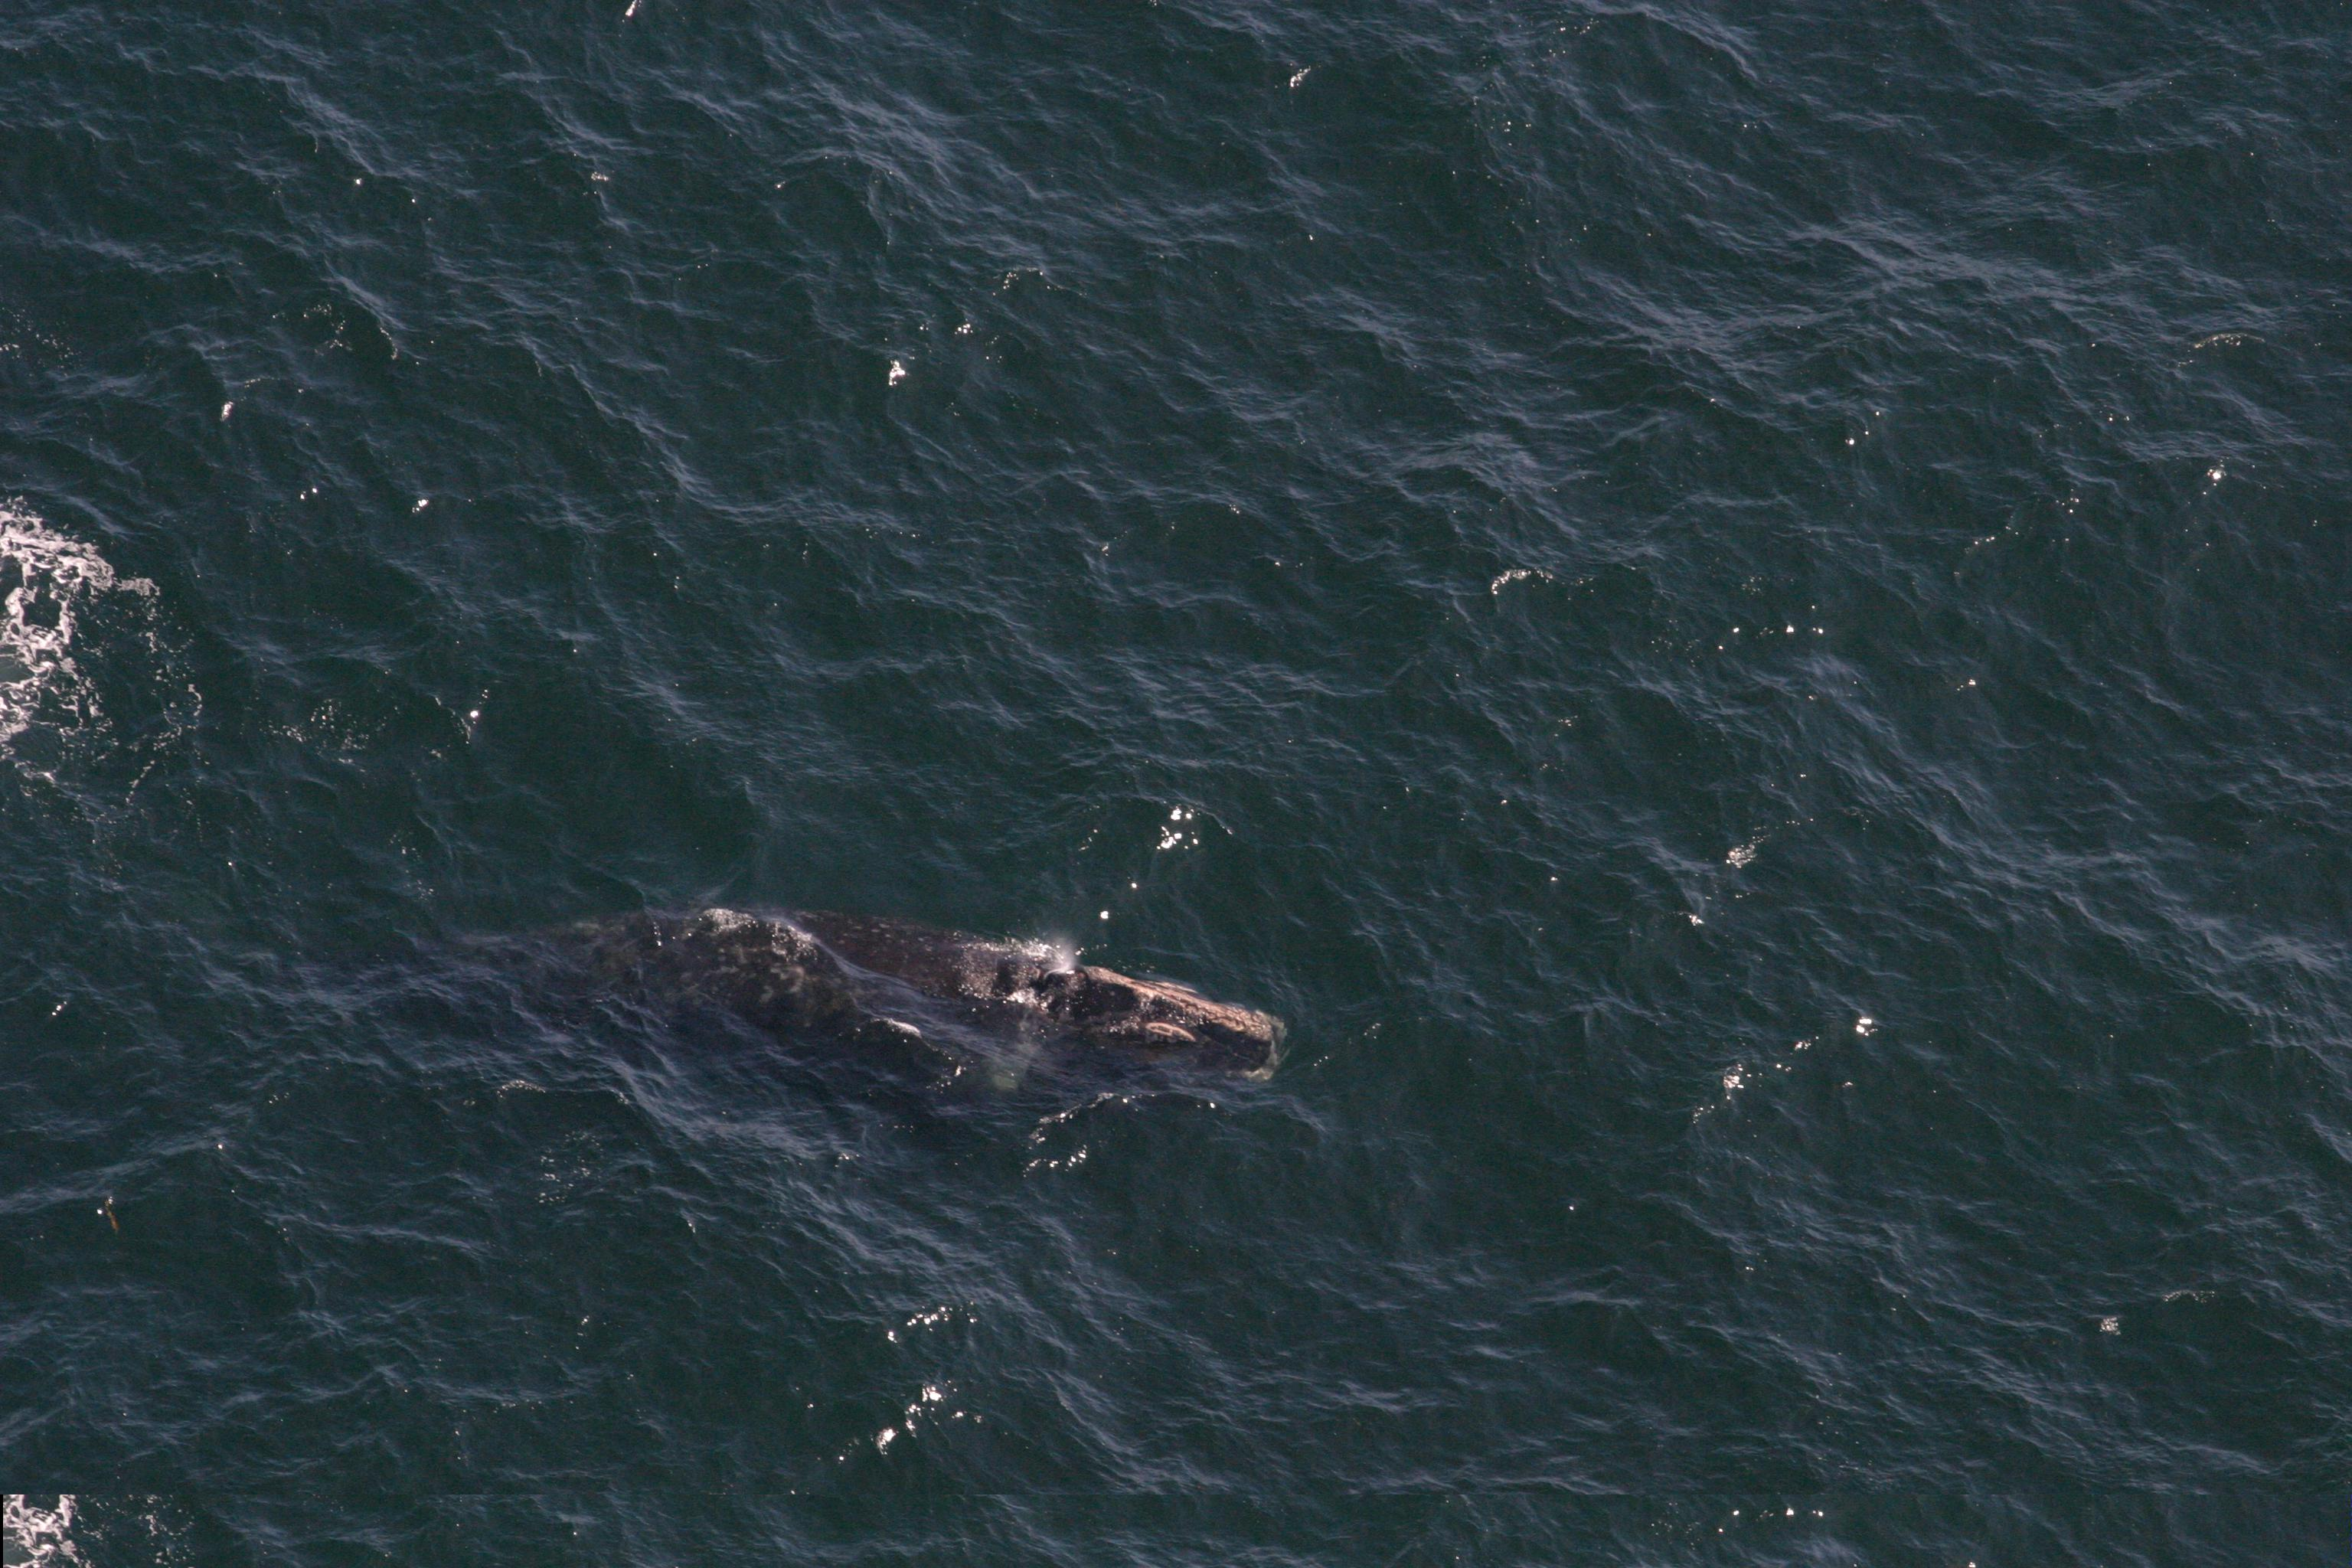
\includegraphics[width=\linewidth]{Images/w_7489}
	\caption{Example of whale from the dataset}
	\label{fig:whale-example}
\end{figure}

Another important thing to note about the dataset is the distribution of unique whales within the training data, an illustration of this can be seen in Figure \ref{fig:whale-frequency}. From this distribution it is notable that some whales are present in more images compared to some of the other whales. The results of the distribution can be seen in Table \ref{table:whale-distribution} where the minimum number of occurrences for a whale is 1 and the maximum is 47 with an average of 10,47 and a standard deviation of 6,8.

\begin{table}
	\centering
	\caption{Unique distribution of whales in the dataset}
	\label{table:whale-distribution}
	\begin{tabularx}{\linewidth}{|X|X|}
		\hline
		Min    & 1     \\ \hline
		Q1     & 5     \\ \hline
		Median & 9     \\ \hline
		Mean   & 10,17 \\ \hline
		Q3     & 14    \\ \hline
		Max    & 47    \\ \hline
		SD     & 6,8   \\ \hline
	\end{tabularx}
\end{table}

\begin{figure}
	\centering
	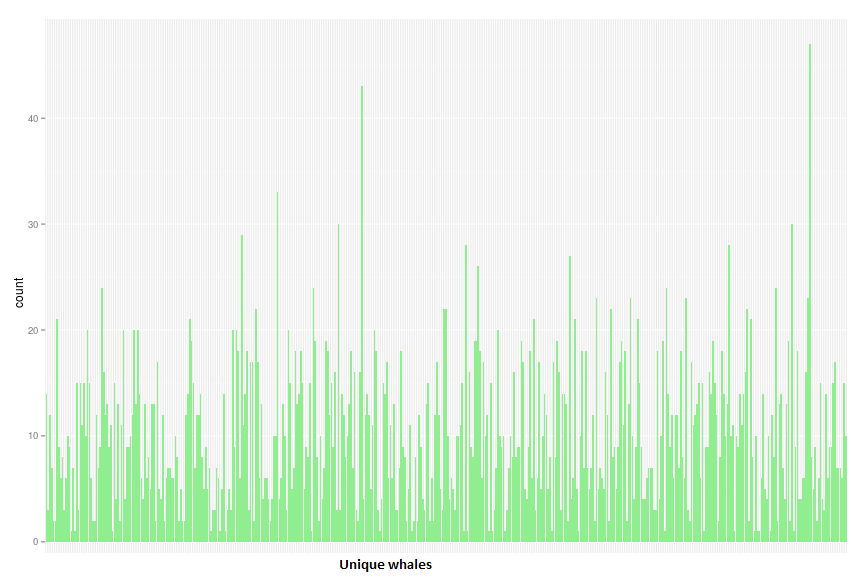
\includegraphics[width=\linewidth]{Images/FrequencyPlot}
	\caption{Frequency of unique whales in the training data}
	\label{fig:whale-frequency}
\end{figure}

\subsection{Methods}
Describes which method has been used in the attempt to correctly classify North Atlantic Right Whales from images.

\subsubsection{Classification Algorithm}
Also known as \emph{Supervised Learning Algorithm}. Classification algorithms have one thing in common, which is that they require data input to be on a similar data structure.
The overall data structure for classifications is that it can contain 1..n observations which each has x amount of data points. For a model, the amount of data points for each observation has to be the same. An example as seen in Table \ref{tab:example data} shows how data could look.
If an observation is missing a value, it can be set to NA\footnote{Not Available} instead. It still has to be present in the structure.

\begin{table}
  \centering
  \caption{Example data}
  \label{tab:example data}
  \begin{tabularx}{\linewidth}{|l|X|X|X|X|} \hline
    obs. & x1 & x2 & x3 & x4 \\ \hline
    1    & 20 & 74 & 84 & 82 \\ \hline
    2    & 52 & 33 & 4  & 36 \\ \hline
    3    & 78 & 55 & 57 & 3  \\ \hline
    4    & 61 & 68 & 65 & 5  \\ \hline
  \end{tabularx}
\end{table}

\paragraph{Decision Tree} is a classification algorithm. 
A decision tree is a binary tree structure where the path in each node is decided based on a split on a given input variable.
This variable split is configured to limit the amount of possible classes down each path. This is done by calculating the entropy (information gain) on each split on a given input variable/feature. This is then done for all input variables. A higher information gain means that a certain split separates different classes better.  
At the end of a path, a leaf contains the class to represent that exact path.
When prediction against a decision tree, that leaf is given as the returned prediction.


\paragraph{Random Forest} is an algorithm which is based upon the decision trees and wisdom of the crowd.
Random Forest spawn multiple decision trees, the algorithm for splitting in the decisions tree in random forest does however differs from how it is done in normal decisions trees.
Random Forest use ``feature bagging'' at each node and then decide for the splitting feature on that subset rather than all the features. This ensures that decision trees is not identical, but offers variety.

\paragraph{Neural Network} is an algorithm as an attempt to mimic how the human brain works.
Neural Networks do however variate from how neurons and connections works in the brain as it contains a link from each node in layer x to each node in layer x + 1. As seen at Figure \ref{fig:neuralnetwork}, a neural network with only an input layer and an output layer is shown and the connections between the nodes. Each input node in the figure is connected to all the output nodes.

\begin{figure}
  \centering
  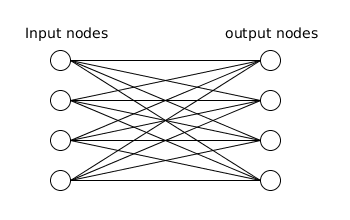
\includegraphics[width=0.7\linewidth]{Images/neuralnetwork}
  \caption{Neural Network with no hidden layers}
  \label{fig:neuralnetwork}
\end{figure}

\subsubsection{Clustering}
Is an \emph{Unsupervised Learning Algorithm} and was used for the preprocessing of the dataset. The specific implementation of the clustering used was K-Means. It splits the data into n clusters and uses euclidean distance to calculate which cluster to add new observations to. Every time at least one data point changes cluster, the center of the clusters are recalculated and the process starts over.

\subsection{Tools and languages}
In this project several different languages and tools have been used. The following list contains a short description of each of them. 

\begin{itemize}
	\item \textit{R} is an programming language licensed under GNU GPL2, used to write the main project \citealp{RLanguage}. In R the following noteworthy packaged have been used
		\begin{itemize}
			\item \textit{cclust} is used for running the clustering \cite{cclust}.
			\item \textit{ggplot2} is used for creating the graphs
			\item \textit{EBImage} is used for image processing \cite{EBI}
		\end{itemize}
	\item \textit{H2O} is a open source data analysis tool written in Java with libraries to be used from Java, Python and R. H20 is created by 0xdata. H2O Have been used for running Random Forest and Neural Network Algorithm \cite{H2O}.
	\item \textit{ImageMagick} is used for handling image processing \cite{ImgMag}
	\item \textit{Java} is used for running some scripts for varies tasks
	\item \textit{Bash} is used for running some scripts for varies tasks
\end{itemize}
